\chapter{Making Planets for Nigel} 
\label{sec:planets}

\begin{definition}[Jeffrey Says]
\setlength{\intextsep}{0pt}%
\setlength{\columnsep}{3pt}%
\begin{wrapfigure}{l}{0.12\textwidth}
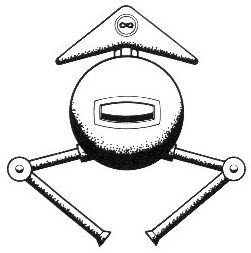
\includegraphics[width=\linewidth]{src/callout/ia.jpg} 
\end{wrapfigure}
\small
Redid the graphics\index{graphics} completely, came up with some really
nice looking metallic\index{metallic} planet\index{planet} structures\index{structures} that I'll probably stick with. Started
to write the \icode{GenPlan} routine\index{routine} that'll generate random planets at will. Good to
have a C64 that can generate planets in its spare time. Wrote pulsation\index{pulsation}
routines for the colours; looks well good with some of the planet\index{planet} structures\index{structures}.
The metallic\index{metallic} look seems to be 'in' at the moment so this first planet\index{planet} will go
down well. There will be five planet\index{planet} surface\index{surface} types in all, I reckon, probably
do one with grass and sea a bit like 'Sheep in Space', cos I did like that one.
It'll be nice to have completely different planet\index{planet} surfaces in top and bottom of
the screen\index{screen}. The neat thing is that all the surfaces have the same basic
structures\index{structures}, all I do is fit different graphics\index{graphics} around each one. 
\end{definition}

When the player presses fire we will leave the title screen and enter the world of the game. Since the
game insists on having a world, that means we are going to have to create one. With enemies, and a ship
that we can move and fire bullets out of. We will also need planets. That sounds like a lot of work to be honest.

Fortunately, making planets is easy. So we can start there. 

When making a planet\index{planet}, ensure you perform each of the following
simple steps in the order given below.

\begin{figure}[H]
  {
    \begin{adjustbox}{width=10cm,center}
      \surface{planets/planet1Charset_Random_Step1.png}
    \end{adjustbox}
  }\caption[]{\textbf{Step One}: Add the sea across the entire surface\index{surface} of the planet\index{planet}, 1024 bytes long.}
\end{figure}

\begin{figure}[H]
  {
    \begin{adjustbox}{width=10cm,center}
      \surface{planets/planet1Charset_Random_Step2.png}
    \end{adjustbox}
  }\caption[]{\textbf{Step Two}: Insert a land mass at least 32 bytes and at most 128 bytes long.}
\end{figure}

\begin{figure}[H]
  {
    \begin{adjustbox}{width=10cm,center}
      \surface{planets/planet1Charset_Random_Step3.png}
    \end{adjustbox}
  }\caption[]{\textbf{Step Three}: Add a random structure\index{structure} every 13 to 29 bytes.}
\end{figure}

\begin{figure}[H]
  {
    \begin{adjustbox}{width=10cm,center}
      \surface{planets/planet1Charset_Random_Step4.png}
    \end{adjustbox}
  }\caption[]{\textbf{Step Four}: Add warp gates at the beginning and end of the planet\index{planet} surface\index{surface}.}
\end{figure}

Now you have not just a layout for one planet\index{planet}, but a layout for all five.

\begin{figure}[H]
  {
      \begin{subfigure}{0.4\textwidth}
        \surface{planets/planet2Charset_Random_Step4.png}
      \end{subfigure}
      \begin{subfigure}{0.4\textwidth}
        \surface{planets/planet3Charset_Random_Step4.png}
      \end{subfigure}
      \begin{subfigure}{0.4\textwidth}
        \surface{planets/planet4Charset_Random_Step4.png}
      \end{subfigure}
      \hspace{2.75cm}
      \begin{subfigure}{0.4\textwidth}
        \surface{planets/planet5Charset_Random_Step4.png}
      \end{subfigure}
  }\caption[]{A layout that will suit all the planets in your life.}
\end{figure}

But making planets isn't all simple steps and big picture decisions. There are also
trifling details for the little people to wrestle with.

\section{Step One: Creating the Sea}

Making a sea is very easy. You come up with a character\index{character} than can be repeated 1024 times to fill the
surface\index{surface} of the planet\index{planet}.

\begin{figure}[H]
{
  \setlength{\tabcolsep}{3.0pt}
  \setlength\cmidrulewidth{\heavyrulewidth} % Make cmidrule = 
    \begin{adjustbox}{width=10cm,center}
  \begin{subfigure}{0.3\textwidth}
  \input{planets/planet1Charset_\$40}
  \end{subfigure}
  \begin{subfigure}{0.3\textwidth}
  \input{planets/planet1Charset_\$42}
  \end{subfigure}
  \end{adjustbox}
}\caption[]{There are two characters used for creating the sea and they're both the same! This will make more sense when
we look at the land, where they are different.}
\end{figure}
\subfile{planets/planet1Charset_sea}

The bit that needs explaining is how you define the character\index{character}. If it was a simple bitmap then we could imagine the
character\index{character} as 8 rows of 8 bits and where a bit is set to 1 you color that pixel in. That is not the case. You can
see how the bits are actually set below:

\begin{figure}[H]
  {
    \setlength{\tabcolsep}{3.0pt}
    \setlength\cmidrulewidth{\heavyrulewidth} % Make cmidrule = 
    \begin{adjustbox}{width=4cm,center}
      \begin{tikzpicture}

        \def\BACKGROUNDONE{brown}
        \def\BACKGROUNDTWO{lightblue}
        \def\CHARCOLOR{lightgreen}
        \draw[step=1.0,gray,thin] (0,0) grid (8,8);
        \fill[\BACKGROUNDTWO] (2,5) rectangle ++ (1,1);
        \fill[\BACKGROUNDTWO] (3,5) rectangle ++ (1,1);
        \fill[\BACKGROUNDTWO] (6,4) rectangle ++ (1,1);
        \fill[\BACKGROUNDTWO] (7,4) rectangle ++ (1,1);
        \fill[\BACKGROUNDTWO] (0,3) rectangle ++ (1,1);
        \fill[\BACKGROUNDTWO] (1,3) rectangle ++ (1,1);
        \fill[\BACKGROUNDTWO] (4,3) rectangle ++ (1,1);
        \fill[\BACKGROUNDTWO] (5,3) rectangle ++ (1,1);
        \fill[\BACKGROUNDTWO] (6,3) rectangle ++ (1,1);
        \fill[\BACKGROUNDTWO] (7,3) rectangle ++ (1,1);
        \fill[\BACKGROUNDTWO] (0,2) rectangle ++ (1,1);
        \fill[\BACKGROUNDTWO] (1,2) rectangle ++ (1,1);
        \fill[\BACKGROUNDTWO] (2,2) rectangle ++ (1,1);
        \fill[\BACKGROUNDTWO] (3,2) rectangle ++ (1,1);
        \fill[\BACKGROUNDTWO] (4,2) rectangle ++ (1,1);
        \fill[\BACKGROUNDTWO] (5,2) rectangle ++ (1,1);
        \fill[\BACKGROUNDTWO] (6,2) rectangle ++ (1,1);
        \fill[\BACKGROUNDTWO] (7,2) rectangle ++ (1,1);
        \fill[\BACKGROUNDTWO] (0,1) rectangle ++ (1,1);
        \fill[\BACKGROUNDTWO] (1,1) rectangle ++ (1,1);
        \fill[\BACKGROUNDTWO] (2,1) rectangle ++ (1,1);
        \fill[\BACKGROUNDTWO] (3,1) rectangle ++ (1,1);
        \fill[\BACKGROUNDTWO] (4,1) rectangle ++ (1,1);
        \fill[\BACKGROUNDTWO] (5,1) rectangle ++ (1,1);
        \fill[\BACKGROUNDTWO] (6,1) rectangle ++ (1,1);
        \fill[\BACKGROUNDTWO] (7,1) rectangle ++ (1,1);
        \fill[\BACKGROUNDTWO] (0,0) rectangle ++ (1,1);
        \fill[\BACKGROUNDTWO] (1,0) rectangle ++ (1,1);
        \fill[\BACKGROUNDTWO] (2,0) rectangle ++ (1,1);
        \fill[\BACKGROUNDTWO] (3,0) rectangle ++ (1,1);
        \fill[\BACKGROUNDTWO] (4,0) rectangle ++ (1,1);
        \fill[\BACKGROUNDTWO] (5,0) rectangle ++ (1,1);
        \fill[\BACKGROUNDTWO] (6,0) rectangle ++ (1,1);
        \fill[\BACKGROUNDTWO] (7,0) rectangle ++ (1,1);
        \node[matrix of math nodes,anchor=south west,inner sep=0pt,
              nodes={draw,minimum size=1cm,anchor=center},
              column sep=-\pgflinewidth,row sep=-\pgflinewidth]
              {0 & 0  & 0 & 0 & 0 & 0 & 0 & 0\\
               0 & 0  & 0 & 0 & 0 & 0 & 0 & 0\\
               0 & 0  & 1 & 0 & 0 & 0 & 0 & 0\\
               0 & 0  & 0 & 0 & 0 & 0 & 1 & 0\\
               1 & 0  & 0 & 0 & 1 & 0 & 1 & 0\\
               1 & 0  & 1 & 0 & 1 & 0 & 1 & 0\\
               1 & 0  & 1 & 0 & 1 & 0 & 1 & 0\\
               1 & 0  & 1 & 0 & 1 & 0 & 1 & 0\\};

      \end{tikzpicture}
    \end{adjustbox}
  }\caption{planet1Charset\index{planet1Charset} \$40 representing a tile of sea.}
\end{figure}

Look closely at the picture above and you should see how it works. What is happening is that we fill
two adjacent cells with blue when together they form the value \icode{10}. So
we create graphic characters not with a simple bit-map but with a map of bit pairs. Each pair of bits is treated as a
unit giving us four units on each row. Maybe it's intuitively obvious that \icode{00}
means 'blank' or 'background\index{background}' but I've pointed that out to you now just in case.

\lstset{style=6502Style}
\begin{lstlisting}[escapechar=\%,caption=Character \icode{\$40} representing the sea as it is defined in the source code. A full eight bytes are required
to define each character\index{character}\, so not cheap.]
planet1Charset%\index{planet1Charset}%
        .BYTE $00,       ; 00000000           
        .BYTE $00,       ; 00000000           
        .BYTE $20,       ; 00100000     *     
        .BYTE $02,       ; 00000010         * 
        .BYTE $8A,       ; 10001010   *   * * 
        .BYTE $AA,       ; 10101010   * * * * 
        .BYTE $AA,       ; 10101010   * * * * 
        .BYTE $AA        ; 10101010   * * * * 
\end{lstlisting}

Is that all there is to it? No. Before we look at how me might color things other than blue, let's look at how we color them
with the big blue brush we have so far. The first thing we do is clear down the entire surface\index{surface} of the planet\index{planet}:

\begin{lstlisting}[escapechar=\%,caption=The surface\index{surface} data is stored from \icode{\$8000} to \icode{\$8FFF}. This code overwrites it all with 
the value \$60\, which is an empty bitmap.]
        ; Clear down the planet%\index{planet}% surface%\index{surface}% data from $8000 to $8FFF.
        ; There are 4 layers:
        ; Top Layer:    $8000 to $83FF - 256 bytes 
        ; Second Layer: $8400 to $87FF - 256 bytes 
        ; Third Layer:  $8800 to $8BFF - 256 bytes 
        ; Bottom Layer: $8C00 to $8FFF - 256 bytes 
        LDY #$00
ClearPlanetHiPtrs%\index{ClearPlanetHiPtrs}%   
        ; $60 is an empty character%\index{character}% and gets written to the entire
        ; range from $8000 to $8FFF.
        LDA #$60
ClearPlanetLoPtrs%\index{ClearPlanetLoPtrs}%   
        STA (planetSurfaceDataPtrLo%\index{planetSurfaceDataPtrLo}%),Y
        DEY
        BNE ClearPlanetLoPtrs%\index{ClearPlanetLoPtrs}%
        INC planetSurfaceDataPtrHi%\index{planetSurfaceDataPtrHi}%
        LDA planetSurfaceDataPtrHi%\index{planetSurfaceDataPtrHi}%
        CMP (#>planetSurfaceData%\index{planetSurfaceData}%%\index{planetSurfaceData%\index{planetSurfaceData}%}%) + $10
        BNE ClearPlanetHiPtrs%\index{ClearPlanetHiPtrs}%
\end{lstlisting}

\begin{lstlisting}[caption=The empty character\index{character} bit map (all zeroes) used to overwrite the surface\index{surface} before populating it.,escapechar=\%]
        .BYTE $00,       ; 00000000           
        .BYTE $00,       ; 00000000           
        .BYTE $00,       ; 00000000           
        .BYTE $00,       ; 00000000           
        .BYTE $00,       ; 00000000           
        .BYTE $00,       ; 00000000           
        .BYTE $00,       ; 00000000           
        .BYTE $00        ; 00000000           
\end{lstlisting}

With the planet\index{planet} surface\index{surface} cleared out (overwritten with all \icode{\$60}s) we can now.. overwrite it all again with sequences of
\icode{\$40,\$42}. No, that's not right. We're only overwriting the bottom layer - the surface\index{surface} layer - this time. This is the
layer that contains the land and/or sea and it lives between \icode{\$8C00} and \icode{\$8FFF} which if your hexadecimal
arithmetic is better than mine you will realize is 1024 bytes (\icode{\$400} in hex).

\begin{lstlisting}[escapechar=\%,caption=Filling the entire bottom surface\index{surface} of the planet\index{planet} with \icode{\$40,\$42}\, which gives us the sea. Our next step is
to overwrite some of this with land.]
        ; Fill $8C00 to $8FFF with a $40,$42 pattern%\index{pattern}%. These are the
        ; character%\index{character}% values that represent 'sea' on the planet%\index{planet}%.
        LDA #$8C
        STA planetSurfaceDataPtrHi%\index{planetSurfaceDataPtrHi}%
WriteSeaLoop%\index{WriteSeaLoop}%   
        LDA #$40
        STA (planetSurfaceDataPtrLo%\index{planetSurfaceDataPtrLo}%),Y
        LDA #$42
        INY
        STA (planetSurfaceDataPtrLo%\index{planetSurfaceDataPtrLo}%),Y
        DEY
        ; Move the pointers%\index{pointers}% forward by 2 bytes
        LDA planetSurfaceDataPtrLo%\index{planetSurfaceDataPtrLo}%
        CLC
        ADC #$02
        STA planetSurfaceDataPtrLo%\index{planetSurfaceDataPtrLo}%
        LDA planetSurfaceDataPtrHi%\index{planetSurfaceDataPtrHi}%
        ADC #$00
        STA planetSurfaceDataPtrHi%\index{planetSurfaceDataPtrHi}%
        ; Loop until $8FFF
        CMP #$90
        BNE WriteSeaLoop%\index{WriteSeaLoop}%
\end{lstlisting}

\subfile{planets/planet1Charset_SeaAgain}

\section{Step Two: Creating the Land}

Is that all there is to it? Painting things with blue? No. 

There are other possible values aside from \icode{10} and \icode{00} that we
could use to paint colors. We could also have \icode{11} and \icode{01}. This
is useful since we want to color things in with more than one color. We have
blue assigned to \icode{10} on Planet 1, while for the land we can use two
other colors: \icode{11} which we will assign 'green' and \icode{01} which we
will assign 'brown'. We can assign whatever colors we like but we can only
choose three, not counting the background\index{background}. This is the kind of limitation you
run into when you only allow two bits for assigning possible colors.

\begin{figure}[H]
{
  \setlength{\tabcolsep}{3.0pt}
  \setlength\cmidrulewidth{\heavyrulewidth} % Make cmidrule = 
    \begin{adjustbox}{width=10cm,center}
  \begin{subfigure}{0.3\textwidth}
  \input{planets/planet1Charset_\$41_bits}
  \end{subfigure}
  \begin{subfigure}{0.3\textwidth}
  \input{planets/planet1Charset_\$43_bits}
  \end{subfigure}
  \end{adjustbox}
}\caption[]{Planet 1 Land uses two different characters that alternate to generate the land surface\index{surface}.}
\end{figure}
\subfile{planets/planet1Charset_land}

The location and length of the landmass is randomly generated with a couple of constraints:
it must be at least 128 bytes  and not more than 256 bytes from the start of surface\index{surface} and it must be at least 32 bytes
and not more than 150 bytes long. The result is that the planet\index{planet} surface\index{surface} will be mostly sea
since the entire surface\index{surface} is 1024 bytes long.

Picking a random number between 128 and 256 is slightly convoluted in assembly:

\begin{lstlisting}[caption=Convoluted.,escapechar=\%]
        ; Get a random number between 0 and 256 and store
        ; in A.
        JSR PutProceduralByteInAccumulatorRegister%\index{PutProceduralByteInAccumulatorRegister}%
        ; Ensure the random number is between 128 and 256.
        AND #$7F ; e.g. $92 becomes $12.
        CLC      ; Clear the carry so addition doesn't overflow%\index{overflow}%.
        ADC #$7F ; e.g. Adding $7F to $12 gives $91 (145).
        ; Store the result.
        STA charSetDataPtrHi%\index{charSetDataPtrHi}%
\end{lstlisting}

With a random start position selected, a similar convolution is performed to choose the length of the land mass:

\begin{lstlisting}[caption=A convolution.,escapechar=\%]
        ; Randomly generate the length of the land section, but
        ; make it at least 32 bytes and not more than 150.
        JSR PutProceduralByteInAccumulatorRegister%\index{PutProceduralByteInAccumulatorRegister}%
        AND #$7F ; Random number between 0 and 128
        CLC
        ADC #$20 ; Add 32
        STA planetSurfaceDataPtrLo%\index{planetSurfaceDataPtrLo}%

\end{lstlisting}

Since the random number we get can be anything between \icode{\$00 - \$FF} (i.e. 0 and 255) and we want a number
that's between 0 and 128 we need to do a bitwise \icode{AND} to mask out Bit 7 which by itself is 128.
\clearpage
\begin{definition}[A Neat Little Trick]
\setlength{\intextsep}{0pt}%
\setlength{\columnsep}{3pt}%
\begin{wrapfigure}{l}{0.12\textwidth}
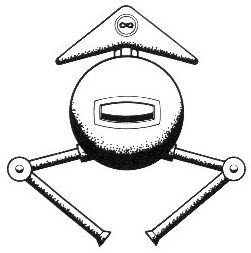
\includegraphics[width=\linewidth]{src/callout/ia.jpg} 
\end{wrapfigure}
\small

This little snippet's job is to return a quasi-random byte for use in the planet\index{planet} generation
routines. To achieve this, it does something quite fiendish that is more or less unhead of in modern
programming: it mutates itself.

\begin{lstlisting}[caption=Neat.,escapechar=\%]
PutProceduralByteInAccumulatorRegister
randomIntToIncrement  =*+$01
        LDA randomPlanetData
        INC randomIntToIncrement
        RTS
\end{lstlisting}

When called for the first time it loads a value from the address at \icode{randomPlanetData\index{randomPlanetData}} to the accumulator. On first
run \icode{randomPlanetData\index{randomPlanetData}} points to the address \icode{\$9ABB} which contains the value \icode{\$42}:

\begin{lstlisting}[caption=Not Quite Random Bytes,escapechar=\%]
randomPlanetData%\index{randomPlanetData}%
        .BYTE $42,$E4,$3F,$94,$4E,$29,$B0,$59
        .BYTE $2C,$FE,$7F,$B2,$40,$9B,$63,$2B
\end{lstlisting}
Before returning this value as its result it alters itself by changing
\icode{randomPlanetData\index{randomPlanetData}} to reference \icode{\$9ABC} (\icode{INC
randomIntToIncrement\index{randomIntToIncrement}}). In other words, it increments the pointer\index{pointer}. In the
assembly listing we make \icode{randomIntToIncrement\index{randomIntToIncrement}} reference the position
that holds \icode{randomPlanetData\index{randomPlanetData}} by positioning it one byte before and
adding a 1 to shift is reference beyond the byte holding \icode{LDA} to
\icode{randomPlanetData\index{randomPlanetData}}.

Every time the routine\index{routine} is called it increments the reference again so that the next time it will pick up whatever
lies in the bytes beyond \icode{9ABB}. The results it returns are never truly random, but random enough
to permit the procedural\index{procedural} generation of planets that they're used for.
\end{definition}
\begin{figure}[H]
  {
    \setlength{\tabcolsep}{3.0pt}
    \setlength\cmidrulewidth{\heavyrulewidth} % Make cmidrule = 
    \begin{adjustbox}{width=10cm,center}

      \begin{tabular}{rllllllll}
        \toprule
        Byte & Bit 7 & Bit 6 & Bit 5 & Bit 4 & Bit 3 & Bit 2 & Bit 1 & Bit 0        \\
        \midrule
        \$FC & 1 & 1 & 1 & 1 & 1 & 1 & 0 & 0 \\
        \$7F & 0 & 1 & 1 & 1 & 1 & 1 & 1 & 1 \\
        \midrule
        Result; \$7C & 0 & 1 & 1 & 1 & 1 & 1 & 0 & 0 \\
        \addlinespace
        \bottomrule
      \end{tabular}

    \end{adjustbox}

  }\caption*{AND'ing \$FC and \$7F gives \$7C (124).}
\end{figure}

With the position and length selected we can start laying turf. We don't just plop down our basic land tiles. Posh
and proper means giving the shore of the land its own look and feel. This we have in the characters \icode{\$5C} and
\icode{\$5E} in our character\index{character} set: 

\begin{figure}[H]
{
  \setlength{\tabcolsep}{3.0pt}
  \setlength\cmidrulewidth{\heavyrulewidth} % Make cmidrule = 
    \begin{adjustbox}{width=15cm,center}
  \begin{subfigure}{0.3\textwidth}
  \input{planets/tilesheets/planet1Charset_tilesheet_\$5C}
  \end{subfigure}
  \begin{subfigure}{0.3\textwidth}
  \input{planets/tilesheets/planet1Charset_tilesheet_\$5E}
  \end{subfigure}
  \begin{subfigure}{0.3\textwidth}
  \input{planets/tilesheets/planet1Charset_tilesheet_\$5D}
  \end{subfigure}
  \begin{subfigure}{0.3\textwidth}
  \input{planets/tilesheets/planet1Charset_tilesheet_\$5F}
  \end{subfigure}
  \end{adjustbox}
}\caption[]{Character tiles for the left shore (\$5C,\$5E) and the right shore (\$5D,\$5F).}
\end{figure}

Now we can put the rest of the land down:

\begin{lstlisting}[caption=Write pairs of \icode{\$41,\$43} for the main land mass.,escapechar=\%]
; Draw the land from the randomly chosen position for up to
; 150 bytes, depending on the randomly chosen length of the land
; chosen above and storedin planetSurfaceDataPtrLo%\index{planetSurfaceDataPtrLo}%.
DrawLandMassLoop%\index{DrawLandMassLoop}%   
        INC charSetDataPtrHi%\index{charSetDataPtrHi}%
        BNE b7420

        INC charSetDataPtrLo%\index{charSetDataPtrLo}%
b7420   JSR StoreRandomPositionInPlanetInPlanetPtr%\index{StoreRandomPositionInPlanetInPlanetPtr}%
        LDY #$00
        LDA #$41
        STA (planetPtrLo%\index{planetPtrLo}%),Y
        LDA #$43
        INY
        STA (planetPtrLo%\index{planetPtrLo}%),Y
        DEC planetSurfaceDataPtrLo%\index{planetSurfaceDataPtrLo}%
        BNE DrawLandMassLoop%\index{DrawLandMassLoop}%
\end{lstlisting}

And finally the right shore:

\begin{lstlisting}[caption=Drawing the right hand shore..,escapechar=\%]
        ; Draw the right short of the land, represented by the chars in
        ; $5D/$5F.
        INY
        LDA #$5D
        STA (planetPtrLo%\index{planetPtrLo}%),Y
        LDA #$5F
        INY
        STA (planetPtrLo%\index{planetPtrLo}%),Y
\end{lstlisting}


\section{Step Three: Structures Structures Structures}
The routines for adding structures\index{structures} to the planet\index{planet} are an opportunity to observe some assembly language cleverness.
For each structure\index{structure} we draw we have to decide two things: where to drop it on the surface\index{surface} and what type of structure\index{structure}
to draw. Apart from the Warp Gates, there are four structure\index{structure} types available. 

\begin{figure}[H]
  {
    \setlength{\tabcolsep}{3.0pt}
    \setlength\cmidrulewidth{\heavyrulewidth} % Make cmidrule = 
    \begin{adjustbox}{width=15cm,center}
      \begin{subfigure}{0.3\textwidth}
        \input{planets/planet1Charset_littleStructureData}
      \end{subfigure}
      \begin{subfigure}{0.3\textwidth}
        \input{planets/planet1Charset_mediumStructureData}
      \end{subfigure}
      \begin{subfigure}{0.3\textwidth}
        \input{planets/planet1Charset_nextLargestStructure}
      \end{subfigure}
      \begin{subfigure}{0.3\textwidth}
        \input{planets/planet1Charset_largestStructureData}
      \end{subfigure}
    \end{adjustbox}
  }\caption[]{The four possible structure\index{structure} types for Planet 1.}
\end{figure}

\begin{figure}[H]
  {
    \setlength{\tabcolsep}{3.0pt}
    \setlength\cmidrulewidth{\heavyrulewidth} % Make cmidrule = 
    \begin{adjustbox}{width=15cm,center}
      \begin{subfigure}{0.3\textwidth}
        \input{planets/planet2Charset_littleStructureData}
      \end{subfigure}
      \begin{subfigure}{0.3\textwidth}
        \input{planets/planet2Charset_mediumStructureData}
      \end{subfigure}
      \begin{subfigure}{0.3\textwidth}
        \input{planets/planet2Charset_nextLargestStructure}
      \end{subfigure}
      \begin{subfigure}{0.3\textwidth}
        \input{planets/planet2Charset_largestStructureData}
      \end{subfigure}
    \end{adjustbox}
  }\caption[]{The four possible structure\index{structure} types for Planet 2.}
\end{figure}

You may be getting the sense that there is a sort of economy at work here. The structures\index{structures} are effectively
the same for each planet\index{planet}, but with the textures\index{textures} swapped out. Your intuition is correct, the structures\index{structures}
are only defined once and the same definition is used regardless of which planet\index{planet} we're painting:

\begin{lstlisting}[caption=The definitions of three of the structures\index{structures} above\, each of which serves all five planets.,escapechar=\%]
littleStructureData%\index{littleStructureData}%  .BYTE $45,$47,$FF
                     .BYTE $44,$46,$FE
mediumStructureData%\index{mediumStructureData}%  .BYTE $65,$67,$69,$6B,$FF
                     .BYTE $64,$66,$68,$6A,$FE
largestStructureData%\index{largestStructureData}% .BYTE $41,$43,$51,$53,$41,$43,$FF
                     .BYTE $60,$60,$50,$52,$60,$60,$FF
                     .BYTE $49,$4B,$4D,$4F,$6D,$6F,$FF
                     .BYTE $48,$4A,$4C,$4E,$6C,$6E,$FE
nextLargestStructure%\index{nextLargestStructure}% .BYTE $59,$5B,$FF
                     .BYTE $58,$5A,$FF
                     .BYTE $55,$57,$FF
                     .BYTE $54,$56,$FE
\end{lstlisting}

The \$FF at the end of each line serves as a sentinel\index{sentinel} for the drawing\index{drawing} routine\index{routine} to know that the subsequent bytes
are for the next layer 'up'. The \$FE is a terminator, indicating there is no more data for the structure\index{structure}.

Drawing a structure\index{structure} is relatively straightforward so we'll cover that briefly first. Drawing the littlest
structure\index{structure} provides the most compact example of the technique:

\begin{lstlisting}[caption=The littlest structure\index{structure} has only two layers.,escapechar=\%]
DrawLittleStructure%\index{DrawLittleStructure}%
        ; Start iterating at 0.
        LDX #$00
DrawLSLoop%\index{DrawLSLoop}%
        ; Get the byte in littleStructureData%\index{littleStructureData}% pointed to
        ; by X.
        LDA littleStructureData%\index{littleStructureData}%,X
        ; If we reached the 'end of layer' sentinel%\index{sentinel}%, move
        ; our pointer%\index{pointer}% planetPtrHi%\index{planetPtrHi}% to the next layer. The
        ; BNE 'stays on the same layer' by jumping%\index{jumping}% to
        ; LS_StayonSameLayer%\index{LS\_StayonSameLayer}% if the current byte
        ; is not $FF.
        CMP #$FF
        BNE LS_StayonSameLayer%\index{LS\_StayonSameLayer}%
        ; Switch to the next layer.
        JSR SwitchToNextLayerInPlanet%\index{SwitchToNextLayerInPlanet}%
        ; SwitchToNextLayerInPlanet%\index{SwitchToNextLayerInPlanet}% incremented X for us
        ; so continue looping%\index{looping}%.
        JMP DrawLSLoop%\index{DrawLSLoop}%

LS_StayonSameLayer%\index{LS\_StayonSameLayer}%   
        CMP #$FE
        ; If we read in an $FE, we're done drawing%\index{drawing}%.
        BEQ ReturnFromDrawingStructure%\index{ReturnFromDrawingStructure}%
        STA (planetPtrLo%\index{planetPtrLo}%),Y
        ; Increment Y to the next position to write to.
        INY
        ; Increment X to get the next byte to read in.
        INX
        ; Continue looping%\index{looping}%.
        JMP DrawLSLoop%\index{DrawLSLoop}%
\end{lstlisting}

Given that we're only writing 4 bytes this is a lot of code. As we will see there are separate routines for each
of the structures\index{structures} and unfortunately for our search for evidence of coding genius they're all identical. So this
is a pretty open-and-shut case of code duplication. It would have been more compact to rationalize them down to a single function\index{function}
and use a pointer\index{pointer} to the structure\index{structure} data instead of repeating almost verbatim the same assembly code for each
structure\index{structure}. 

\begin{lstlisting}[escapechar=\%,caption=\icode{DrawMediumStructure\index{DrawMediumStructure}} and \icode{DrawLargestStructure\index{DrawLargestStructure}} are identical to each other\, and to
\icode{DrawLittleStructure\index{DrawLittleStructure}} and \icode{DrawNextLargestStructure\index{DrawNextLargestStructure}}.]
;-------------------------------------------------------
; DrawMediumStructure%\index{DrawMediumStructure}% ($74B1)
;-------------------------------------------------------
DrawMediumStructure%\index{DrawMediumStructure}%
        LDX #$00

DrawMSLoop%\index{DrawMSLoop}%
        LDA mediumStructureData%\index{mediumStructureData}%,X
        CMP #$FF
        BNE b74C0
        JSR SwitchToNextLayerInPlanet%\index{SwitchToNextLayerInPlanet}%
        JMP DrawMSLoop%\index{DrawMSLoop}%

b74C0   CMP #$FE
        BEQ ReturnFromDrawingStructure%\index{ReturnFromDrawingStructure}% ; Return
        STA (planetPtrLo%\index{planetPtrLo}%),Y
        INY
        INX
        JMP DrawMSLoop%\index{DrawMSLoop}%

;-------------------------------------------------------
; DrawLargestStructure%\index{DrawLargestStructure}% ($74CB)
;-------------------------------------------------------
DrawLargestStructure%\index{DrawLargestStructure}%
        LDX #$00

DrawLargeStructureLoop%\index{DrawLargeStructureLoop}%
        LDA largestStructureData%\index{largestStructureData}%,X
        CMP #$FF
        BNE b74DA
        JSR SwitchToNextLayerInPlanet%\index{SwitchToNextLayerInPlanet}%
        JMP DrawLargeStructureLoop%\index{DrawLargeStructureLoop}%

b74DA   CMP #$FE
        BEQ ReturnFromDrawingStructure%\index{ReturnFromDrawingStructure}% ; Return
        STA (planetPtrLo%\index{planetPtrLo}%),Y
        INY
        INX
        JMP DrawLargeStructureLoop%\index{DrawLargeStructureLoop}%
\end{lstlisting}

The cleverness comes a little earlier so let's console ourselves with that. When we've chosen a position to draw
our structure\index{structure} we need to pick a type of structure\index{structure} at random. The secret to this is to store the addresses to our
regrettably repetitive draw routines in a pair of arrays. 


\begin{lstlisting}[escapechar=\%,caption=A 'jump table' containing the addresses to our draw routines. The address for \icode{DrawLittleStructure\index{DrawLittleStructure}}
happens to be \$7486\, so we store \$74 in the first byte of \icode{structureSubRoutineArrayHiPtr\index{structureSubRoutineArrayHiPtr}} and \$86 in the first
byte of \icode{structureSubRoutineArrayLoPtr\index{structureSubRoutineArrayLoPtr}}.]
;Jump table
structureSubRoutineArrayHiPtr%\index{structureSubRoutineArrayHiPtr}% 
 .BYTE >DrawLittleStructure%\index{DrawLittleStructure}%,>DrawMediumStructure%\index{DrawMediumStructure}%
 .BYTE >DrawLargestStructure%\index{DrawLargestStructure}%,>DrawNextLargestStructure%\index{DrawNextLargestStructure}%
structureSubRoutineArrayLoPtr%\index{structureSubRoutineArrayLoPtr}% 
 .BYTE <DrawLittleStructure%\index{DrawLittleStructure}%,<DrawMediumStructure%\index{DrawMediumStructure}%
 .BYTE <DrawLargestStructure%\index{DrawLargestStructure}%,<DrawNextLargestStructure%\index{DrawNextLargestStructure}%
\end{lstlisting}

With this in place our routine\index{routine} consists of getting a random number between 0 and 3, then using that as in index to pick
out a value at the same position from \icode{structureSub\-RoutineArrayLoPtr} and \icode {structureSubRoutineArrayHiPtr\index{structureSubRoutineArrayHiPtr}}.
We then store those values in \icode{structureRoutineLoPtr\index{structureRoutineLoPtr}} and \icode{structureRoutineHiPtr\index{structureRoutineHiPtr}} respectively. We now
have a pointer\index{pointer} to one of our draw routines at \icode{structureRoutineLoPtr\index{structureRoutineLoPtr}} which we can jump to with the simple
command: \icode{JMP (structureRoutineLoPtr\index{structureRoutineLoPtr})}. 


\begin{lstlisting}[caption=\icode{DrawRandomlyChosenStructure\index{DrawRandomlyChosenStructure}} picks a random position and a random draw routine\index{routine} to use at that position.,escapechar=\%]
;---------------------------------------------------------------
; DrawRandomlyChosenStructure%\index{DrawRandomlyChosenStructure}%
;---------------------------------------------------------------
DrawRandomlyChosenStructure%\index{DrawRandomlyChosenStructure}%
        ; Pick a random positio to draw the structure%\index{structure}%
        JSR StoreRandomPositionInPlanetInPlanetPtr%\index{StoreRandomPositionInPlanetInPlanetPtr}%

        ; Run the randomly chose subroutine%\index{subroutine}%, one of:
        ; DrawLittleStructure%\index{DrawLittleStructure}%, DrawMediumStructure%\index{DrawMediumStructure}%,
        ; DrawLargestStructure%\index{DrawLargestStructure}%, DrawNextLargestStructure%\index{DrawNextLargestStructure}%
        ; to draw a structure%\index{structure}% on the planet%\index{planet}% surface%\index{surface}%

        ; Pick a random number between 0 and 3
        JSR PutProceduralByteInAccumulatorRegister%\index{PutProceduralByteInAccumulatorRegister}%
        ; AND'ing with $03 ensures the number is between
        ; 0 and 3.
        AND #$03
        ; Move the number to the X register%\index{register}%.
        TAX
        ; Use the random number to pick and draw a structure%\index{structure}%.
        LDA structureSubRoutineArrayHiPtr%\index{structureSubRoutineArrayHiPtr}%,X
        STA structureRoutineHiPtr%\index{structureRoutineHiPtr}%
        LDA structureSubRoutineArrayLoPtr%\index{structureSubRoutineArrayLoPtr}%,X
        STA structureRoutineLoPtr%\index{structureRoutineLoPtr}%
        ; With the address of the routine%\index{routine}% we've chosen copied
        ; to structureRoutineLoPtr%\index{structureRoutineLoPtr}%, we jump to that address and
        ; run the routine%\index{routine}%.
        JMP (structureRoutineLoPtr%\index{structureRoutineLoPtr}%)
        ; The routine%\index{routine}% contains an 'RTS' so does the returning
        ; for us.
\end{lstlisting}

Rinse and repeat this for the length of the map and we get a surface\index{surface} with sea and land that is dotted with structures\index{structures}
of different types.

\begin{figure}[H]
  {
    \begin{adjustbox}{width=10cm,center}
      \surface{planets/planet3Charset_Random_Step3.png}
    \end{adjustbox}
  }\caption[]{Planet 3 once \icode{DrawRandomlyChosenStructure\index{DrawRandomlyChosenStructure}} has finished its business.}
\end{figure}

\section{Step Four: Add the warp gate}

Our final step is to add the warp gate.
\begin{figure}[H]
  {
    \setlength{\tabcolsep}{3.0pt}
    \setlength\cmidrulewidth{\heavyrulewidth} % Make cmidrule = 
    \begin{adjustbox}{width=15cm,center}
      \begin{subfigure}{0.3\textwidth}
        \input{planets/planet1Charset_warpGateData}
      \end{subfigure}
      \begin{subfigure}{0.3\textwidth}
        \input{planets/planet2Charset_warpGateData}
      \end{subfigure}
      \begin{subfigure}{0.3\textwidth}
        \input{planets/planet3Charset_warpGateData}
      \end{subfigure}
      \begin{subfigure}{0.3\textwidth}
        \input{planets/planet4Charset_warpGateData}
      \end{subfigure}
      \begin{subfigure}{0.3\textwidth}
        \input{planets/planet5Charset_warpGateData}
      \end{subfigure}
    \end{adjustbox}
  }\caption[]{The warp gates on each planet\index{planet}.}
\end{figure}

There's something funny here I haven't figured out yet. The routine\index{routine} for drawing\index{drawing} the warp gate
draws it twice. Yet each level has only one warp gate. Each one gets an initial position of
\$F1 and \$05 respectively. This is used by \icode{StoreRandomPositionInPlanetInPlanetPtr\index{StoreRandomPositionInPlanetInPlanetPtr}} to 
point to a position on the surface\index{surface} where the warp gate is drawn.

\begin{lstlisting}[caption=Why does it draw 2 warp gates when there's only 1? Haven't figured this out yet..,escapechar=\%]
DrawWarpGates%\index{DrawWarpGates}%   
        LDA charSetDataPtrLo%\index{charSetDataPtrLo}%
        BEQ GenerateStructuresLoop%\index{GenerateStructuresLoop}%

        ; Draw a warp gate at the end of the map.
        LDA #$F1
        STA charSetDataPtrHi%\index{charSetDataPtrHi}%

        JSR StoreRandomPositionInPlanetInPlanetPtr%\index{StoreRandomPositionInPlanetInPlanetPtr}%
        JSR DrawWarpGate%\index{DrawWarpGate}%
        DEC charSetDataPtrLo%\index{charSetDataPtrLo}%

        ; Draw a warp gate at the start of the map.
        LDA #$05
        STA charSetDataPtrHi%\index{charSetDataPtrHi}%

        JSR StoreRandomPositionInPlanetInPlanetPtr%\index{StoreRandomPositionInPlanetInPlanetPtr}%
        JSR DrawWarpGate%\index{DrawWarpGate}%
\end{lstlisting}

\begin{figure}[H]
  {
    \begin{adjustbox}{width=10cm,center}
      \begin{subfigure}{0.7\textwidth}
        \surface{planets/planet4Charset_Random_Step4.png}
      \end{subfigure}
      \begin{subfigure}{0.7\textwidth}
        \surface{planets/planet5Charset_Random_Step4.png}
      \end{subfigure}
  \end{adjustbox}
  }\caption[]{The final surfaces for Planets 4 and 5.}
\end{figure}

\section{Inactive Lower Planet}
When the lower planet\index{planet} is inactive a surface\index{surface} with land, sea, and a warp gate is displayed. This doesn't reuse
any of the logic described above. Instead it is generated from some customized data in the routine\index{routine}
\icode{DrawLowerPlanetWhileInactive\index{DrawLowerPlanetWhileInactive}}.

\begin{lstlisting}[caption=Draw the inactive lower planet\index{planet}.,escapechar=\%]
;-----------------------------------------------------------
; DrawLowerPlanetWhileInactive%\index{DrawLowerPlanetWhileInactive}%
; Draws the lower planet%\index{planet}% for the early levels when it isn't
; active yet.
;-----------------------------------------------------------
DrawLowerPlanetWhileInactive%\index{DrawLowerPlanetWhileInactive}%
        LDA lowerPlanetActivated%\index{lowerPlanetActivated}%
        BEQ b6047

        LDX #$28
DrawLowerTextLoop%\index{DrawLowerTextLoop}%   
        LDA textForInactiveLowerPlanet%\index{textForInactiveLowerPlanet}% - $01,X
        AND #$3F
        STA SCREEN_RAM%\index{SCREEN\_RAM}% + LINE18_COL39%\index{LINE18\_COL39}%,X
        LDA #WHITE
        STA COLOR_RAM%\index{COLOR\_RAM}% + LINE18_COL39%\index{LINE18\_COL39}%,X
        DEX
        BNE DrawLowerTextLoop%\index{DrawLowerTextLoop}%

        LDX #$28
DrawInactiveSurfaceLoop%\index{DrawInactiveSurfaceLoop}%   
        LDA surfaceDataInactiveLowerPlanet%\index{surfaceDataInactiveLowerPlanet}%,X
        CLC
        ADC #$40
        STA SCREEN_RAM%\index{SCREEN\_RAM}% + LINE14_COL39%\index{LINE14\_COL39}%,X
        DEX
        BNE DrawInactiveSurfaceLoop%\index{DrawInactiveSurfaceLoop}%

        LDX #$10
DrawWarpGateInactive%\index{DrawWarpGateInactive}%   
        LDY xPosSecondLevelSurfaceInactivePlanet%\index{xPosSecondLevelSurfaceInactivePlanet}%,X
        LDA secondLevelSurfaceDataInactivePlanet%\index{secondLevelSurfaceDataInactivePlanet}%,X
        CLC
        ADC #$40
        STA SCREEN_RAM%\index{SCREEN\_RAM}% + LINE12_COL4%\index{LINE12\_COL4}%,Y
        DEX
        BNE DrawWarpGateInactive%\index{DrawWarpGateInactive}%
        RTS

; The *-$01 is because the array index starts at 1 rather than 0.
xPosSecondLevelSurfaceInactivePlanet%\index{xPosSecondLevelSurfaceInactivePlanet}% =*-$01
       .BYTE $00,$01,$02,$03,$28,$29,$2A,$2B
       .BYTE $50,$51,$52,$53,$78,$79,$7A,$7B
secondLevelSurfaceDataInactivePlanet%\index{secondLevelSurfaceDataInactivePlanet}% =*-$01 
       .BYTE $30,$32,$38,$3A,$31,$33,$39,$3B
       .BYTE $34,$36,$3C,$3E,$35,$37,$3D,$3F
surfaceDataInactiveLowerPlanet%\index{surfaceDataInactiveLowerPlanet}% =*-$01       
       .BYTE $01,$03,$01,$03,$01,$03,$01,$03
       .BYTE $01,$03,$01,$03,$01,$03,$01,$03
       .BYTE $01,$03,$01,$03,$01,$03,$01,$03
       .BYTE $01,$03,$01,$03,$01,$03,$1D,$1F
       .BYTE $00,$02,$00,$02,$00,$02,$00,$02

textForInactiveLowerPlanet%\index{textForInactiveLowerPlanet}%
      .TEXT "  WARP GATE       GILBY   CORE  NOT-CORE%\index{NOT-CORE}%"
\end{lstlisting}


\section{Drawing the Lower Planet}
Drawing the upper planet\index{planet} is all very well. The data is just there and as we have seen it's just a question
of 'writing it to the screen\index{screen}'. For the lower planet\index{planet}, which is just an upside down version of the upper one,
we could store the data all over again, but inverted\index{inverted}. Or we could try something a little more clever,
so let's be clever.

Our clever trick will be to take each character\index{character} definition for the upper planet\index{planet} and shift its bits around
so that we can turn it into an upside down version of the original. This avoids the need to store everything
twice. Instead we store it once for the upper planet\index{planet} and just mutate it for the lower planet\index{planet}.

\begin{figure}[H]
{
  \setlength{\tabcolsep}{3.0pt}
  \setlength\cmidrulewidth{\heavyrulewidth} % Make cmidrule = 
    \begin{adjustbox}{width=10cm,center}
  \begin{subfigure}{0.3\textwidth}
  \input{planets/planet1Charset_\$40_bits}
  \end{subfigure}
  \begin{subfigure}{0.3\textwidth}
  \input{planets/planet1Charset_\$40_bits_inv}
  \end{subfigure}
  \end{adjustbox}
}\caption[]{The character\index{character} set definition for a piece of land and it's topsy-turvy counterpart.}
\end{figure}

Doing this all at once for the full planet\index{planet} would be expensive and there will never be a good time to do it.
So what we'll do instead is make a chutney from this pickle and do the heavy lifting while distracting the
player's attention with an impressive-looking level-entry sequence\index{sequence}.

When the player enters a pair of planets for the first time we'll slowly materialize the planet\index{planet} surfaces
while quietly loading the upper planet\index{planet} data and converting it for the lower planet\index{planet} too. If we make
this entry sequence\index{sequence} long enough we'll have time to populate all 256 bytes of each planet\index{planet}'s surface\index{surface}.

\begin{figure}[H]
    \centering
    \foreach \l in {10, 32, ...,125}
    {
      \includegraphics[width=4cm]{planets/entry_images/entry\l.png}%
    }%
\end{figure}
\begin{figure}[H]
    \centering
    \foreach \l in {125, 147, ...,255}
    {
      \includegraphics[width=4cm]{planets/entry_images/entry\l.png}%
    }%
\caption{The materialization sequence\index{sequence} as we enter a new pair of planets.}
\end{figure}

The trickery takes place in \icode{MaybeDrawLevelEntrySequence\index{MaybeDrawLevelEntrySequence}}, one of the many routines called in
the busiest code junction in the raster interrupt\index{interrupt} used during main game play. Even though the game
isn't properly 'playing' at this point all of the main game code is running during the entry
level sequence\index{sequence} though nearly all of it except for this routine\index{routine} exits early as there is nothing
for most of the routines to do:

\begin{lstlisting}[escapechar=\%,caption=\icode{PerformMainGameUpdate\index{PerformMainGameUpdate}}\, the spaghetti junction handling nearly everything
during main gameplay. We'll see more of this code section later in the book. During the entry level sequence\index{sequence}
it is \icode{MaybeDrawLevelEntrySequence\index{MaybeDrawLevelEntrySequence}} and \icode{PlaySoundEffects\index{PlaySoundEffects}} that do most of the work.]
;-------------------------------------------------------
; PerformMainGameUpdate%\index{PerformMainGameUpdate}%
;-------------------------------------------------------
PerformMainGameUpdate%\index{PerformMainGameUpdate}%
        LDX currentPlanetBackgroundClr1%\index{currentPlanetBackgroundClr1}%
        LDA backgroundColorsForPlanets%\index{backgroundColorsForPlanets}%,X
        STA $D022    ;Background Color 1, Multi-Color%\index{Multi-Color}% Register%\index{Register}% 0
        LDX currentPlanetBackgroundClr2%\index{currentPlanetBackgroundClr2}%
        LDA backgroundColorsForPlanets%\index{backgroundColorsForPlanets}%,X
        STA $D023    ;Background Color 2, Multi-Color%\index{Multi-Color}% Register%\index{Register}% 1

        LDA $D01F    ;Sprite to Background Collision%\index{Collision}% Detect
        STA spriteCollidedWithBackground%\index{spriteCollidedWithBackground}%

        JSR CheckKeyboardInGame%\index{CheckKeyboardInGame}%
        JSR ScrollStarfieldAndThenPlanets%\index{ScrollStarfieldAndThenPlanets}%
        JSR AnimateGilbySpriteMovement
        JSR PerformMainGameProcessing%\index{PerformMainGameProcessing}%
        JSR CheckForLandscapeCollisionAndWarpThenProcessJoystickInput
        JSR PerformGilbyLandingOrJumpingAnimation
        JSR AlsoPerformGilbyLandingOrJumpingAnimation
        JSR MaybeDrawLevelEntrySequence%\index{MaybeDrawLevelEntrySequence}%
        JSR PlaySoundEffects%\index{PlaySoundEffects}%
        JSR FlashBorderAndBackground%\index{FlashBorderAndBackground}%
        JSR UpdateGilbyPositionAndColor
        JSR UpdateAndAnimateAttackShips%\index{UpdateAndAnimateAttackShips}%
        JSR UpdateBulletPositions%\index{UpdateBulletPositions}%
        JSR DrawUpperPlanetAttackShips%\index{DrawUpperPlanetAttackShips}%
        JSR UpdateControlPanelColors%\index{UpdateControlPanelColors}%
        ; Jump into KERNAL's standard interrupt%\index{interrupt}% service routine%\index{routine}% to 
        ; handle keyboard%\index{keyboard}% scan, cursor display etc.
        JMP ReEnterInterrupt%\index{ReEnterInterrupt}% 
        ;Returns%\index{Returns}% From Interrupt%\index{Interrupt}%
\end{lstlisting}

\icode{MaybeDrawLevelEntrySequence\index{MaybeDrawLevelEntrySequence}}'s principal sleight-of-hand is to make it look like it is slowly filling
out the surface\index{surface} of the planets when that is precisely what it is doing. Not just to look fancy, but because
inverting the tiles of the lower planet\index{planet} takes a bit of CPU time and would result in the player starting a blank screen\index{screen}
for quite a long time if we tried to do it all at once.

The routine\index{routine} maintains a counter from 0 to 255 and every time it is visited it increments this counter and uses it
to pick part of a tile in the charset\index{charset} to populate. The thing to remember here is that it is not actually painting the planet\index{planet}
itself - rather it is slowly filling out the character\index{character} set containing the tiles that define the textures\index{textures} on the planet\index{planet}.
The game already knows which tiles it wants to put where - it just doesn't yet know what they look like. If we maintained
separate copies of the upper planet\index{planet} and lower planet\index{planet} tiles we could just give them to the routine\index{routine} and painting would be easy.
But because we don't have a copy of the lower planet\index{planet} tiles we have to generate them on the fly and resort to this
bit of entry level sequence\index{sequence} trickery.

Since there are 8 bytes in each character\index{character} set definition, each represeting a line in the tile, 
each visit to this routine\index{routine} updates just one line in one tile. There are 32 tiles in total so 256 visits to the routine\index{routine}
during the entry sequence\index{sequence} will be enough to fill out the tileset completely. This allows
us to fill out the tile set in a random-looking way and is responsible for the materialization effect.

The first part of the \icode{MaybeDrawLevelEntrySequence\index{MaybeDrawLevelEntrySequence}} is the easy part. We just pick the byte we're going to fill
at this visit from a jumbled array of every value between 0 and 255 stored in \icode{sourceOfSeedBytes\index{sourceOfSeedBytes}}. This jumbled
sequence\index{sequence} is the source of the random-looking nature of the materialization.

\begin{lstlisting}[escapechar=\%,caption=The start of \icode{MaybeDrawLevelEntrySequence\index{MaybeDrawLevelEntrySequence}}. As long as \icode{levelEntrySequenceActive\index{levelEntrySequenceActive}}
is non-zero\, \icode{DrawLevelEntrySequence\index{DrawLevelEntrySequence}} will run.]
MaybeDrawLevelEntrySequence%\index{MaybeDrawLevelEntrySequence}%
        LDA levelEntrySequenceActive%\index{levelEntrySequenceActive}%
        BNE DrawLevelEntrySequence%\index{DrawLevelEntrySequence}%
ReturnFromEntrySequence%\index{ReturnFromEntrySequence}%   
        RTS

DrawLevelEntrySequence%\index{DrawLevelEntrySequence}%   
        LDX entryLevelSequenceCounter%\index{entryLevelSequenceCounter}%
        ; 'Y' becomes our 'random' index into the
        ; character%\index{character}% set definition picking one of its
        ; 256 bytes to populate a line in one of the tiles.
        LDY sourceOfSeedBytes%\index{sourceOfSeedBytes}%,X

        ; Pointers to the character%\index{character}% set used for the
        ; current planet%\index{planet}%.
        LDA currentTopPlanetDataLoPtr%\index{currentTopPlanetDataLoPtr}%
        STA planetSurfaceDataPtrLo%\index{planetSurfaceDataPtrLo}%
        LDA currentTopPlanetDataHiPtr%\index{currentTopPlanetDataHiPtr}%
        STA planetSurfaceDataPtrHi%\index{planetSurfaceDataPtrHi}%

        ; The easy part, just copy part of the tile
        ; for the upper planet%\index{planet}% to where it needs to go.
        LDA (planetSurfaceDataPtrLo%\index{planetSurfaceDataPtrLo}%),Y
        STA upperPlanetSurfaceCharset%\index{upperPlanetSurfaceCharset}%,Y

        INC planetSurfaceDataPtrHi%\index{planetSurfaceDataPtrHi}%
        ; Likewise for the character%\index{character}% set data used to 
        ; define the heads up display.
        LDA (planetSurfaceDataPtrLo%\index{planetSurfaceDataPtrLo}%),Y
        STA upperPlanetHUDCharset%\index{upperPlanetHUDCharset}%,Y

        JSR InvertSurfaceDataForLowerPlanet%\index{InvertSurfaceDataForLowerPlanet}%
\end{lstlisting}


This all just copying and pasting so far. We're slowly populating the tiles for the current upper planet\index{planet} without doing
anything computationally intensive. The very last statement is where start work on the lower planet\index{planet}, and that's where
the sorcery starts. In \icode{InvertSurfaceDataForLowerPlanet\index{InvertSurfaceDataForLowerPlanet}} we repoint ourselves to the data for the lower planet\index{planet}
and use a routine\index{routine} called \icode{InvertCharacter\index{InvertCharacter}} to the do the actual turning of the byte upside-down:

\begin{lstlisting}[caption=\icode{InvertSurfaceDataForLowerPlanet\index{InvertSurfaceDataForLowerPlanet}}.,escapechar=\%]
InvertSurfaceDataForLowerPlanet%\index{InvertSurfaceDataForLowerPlanet}%
        LDA currentBottomPlanetDataLoPtr%\index{currentBottomPlanetDataLoPtr}%
        STA planetSurfaceDataPtrLo%\index{planetSurfaceDataPtrLo}%
        LDA currentBottomPlanetDataHiPtr%\index{currentBottomPlanetDataHiPtr}%
        STA planetSurfaceDataPtrHi%\index{planetSurfaceDataPtrHi}%

        ; This is the routine%\index{routine}% that does the actual inversion.
        ; Everything below and above is managing the copy/paste
        ; of the inverted%\index{inverted}% character%\index{character}% into the appropriate position
        ; in lowerPlanetSurfaceCharset%\index{lowerPlanetSurfaceCharset}%.
        JSR InvertCharacter%\index{InvertCharacter}%

        LDA invertedCharToDraw%\index{invertedCharToDraw}%
        ; Note that 'X' was updated by InvertCharacter%\index{InvertCharacter}%
        STA lowerPlanetSurfaceCharset%\index{lowerPlanetSurfaceCharset}%,X
        INC planetSurfaceDataPtrHi%\index{planetSurfaceDataPtrHi}%

        ; Same as above, but for the charset%\index{charset}% used in the panel.
        JSR InvertCharacter%\index{InvertCharacter}%
        LDA invertedCharToDraw%\index{invertedCharToDraw}%
        ; Note that 'X' was updated by InvertCharacter%\index{InvertCharacter}%
        STA lowerPlanetHUDCharset%\index{lowerPlanetHUDCharset}%,X

        RTS
\end{lstlisting}

The approach taken by \icode{InvertCharacter\index{InvertCharacter}} is two-fold: it has to reverse the chosen byte left to right and 
it also it has to move the byte to its appropriate position in the 8 byte sequence\index{sequence}.

\begin{figure}[H]
{
  \setlength{\tabcolsep}{3.0pt}
  \setlength\cmidrulewidth{\heavyrulewidth} % Make cmidrule = 
    \begin{adjustbox}{width=10cm,center}
  \begin{subfigure}{0.3\textwidth}
  \input{planets/planet1Charset_\$40_bits_1}
  \end{subfigure}
  \begin{subfigure}{0.3\textwidth}
  \input{planets/planet1Charset_\$40_bits_inv_1}
  \end{subfigure}
  \end{adjustbox}
}\caption[]{Inverting \icode{00100000} means transforming it to \icode{00001000} and moving it from position 3 in the
  8 byte character\index{character} set definition to position 5.}
\end{figure}

\subsection{Flipping the Byte}
The first of these requirements is the more elaborate of the two. We need to look at each of the four bit-pairs in the
byte and move it to its corresponding 'inverted\index{inverted}' position in the byte. So in a way we treat one half of they byte as
a mirror of the other and move the bit pair there as in the following examples.

\begin{figure}[H]
  {
    \setlength{\tabcolsep}{3.0pt}
    \setlength\cmidrulewidth{\lightrulewidth} % Make cmidrule = 
    \begin{adjustbox}{width=10cm,center}
      \begin{tikzpicture}
        \draw[step=1.0,gray,thin] (0,0) grid (1,1);
        \node[matrix of math nodes,anchor=south west,inner sep=0pt,
        nodes={draw,minimum size=1cm,anchor=center},
        column sep=-\pgflinewidth,row sep=-\pgflinewidth,font=\huge\ttfamily]
        {
        1 & 0  & 0 & 0 & 0 & 0 & 0 & 0\\
        };
      \end{tikzpicture}
      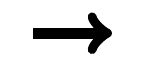
\begin{tikzpicture}
        \draw[->,line width=4pt] (0,0) to (1,0);
      \end{tikzpicture}
      \begin{tikzpicture}
        \draw[step=1.0,gray,thin] (0,0) grid (1,1);
        \node[matrix of math nodes,anchor=south west,inner sep=0pt,
        nodes={draw,minimum size=1cm,anchor=center},
        column sep=-\pgflinewidth,row sep=-\pgflinewidth,font=\huge\ttfamily]
        {
        0 & 0  & 0 & 0 & 0 & 0 & 1 & 0\\
        };
      \end{tikzpicture}
    \end{adjustbox}
    \begin{adjustbox}{width=10cm,center}
      \begin{tikzpicture}
        \draw[step=1.0,gray,thin] (0,0) grid (1,1);
        \node[matrix of math nodes,anchor=south west,inner sep=0pt,
        nodes={draw,minimum size=1cm,anchor=center},
        column sep=-\pgflinewidth,row sep=-\pgflinewidth,font=\huge\ttfamily]
        {
        0 & 0  & 1 & 0 & 0 & 0 & 0 & 0\\
        };
      \end{tikzpicture}
      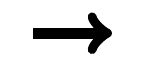
\begin{tikzpicture}
        \draw[->,line width=4pt] (0,0) to (1,0);
      \end{tikzpicture}
      \begin{tikzpicture}
        \draw[step=1.0,gray,thin] (0,0) grid (1,1);
        \node[matrix of math nodes,anchor=south west,inner sep=0pt,
        nodes={draw,minimum size=1cm,anchor=center},
        column sep=-\pgflinewidth,row sep=-\pgflinewidth,font=\huge\ttfamily]
        {
        0 & 0  & 0 & 0 & 1 & 0 & 0 & 0\\
        };
      \end{tikzpicture}
    \end{adjustbox}
  }\caption{Examples of the inversion operation.}
\end{figure}

The way to do through a combination of bit-shifting\index{shifting} and masking. This is what the code
responsible looks like. We'll break it down.

\begin{lstlisting}[caption=\icode{InvertSurfaceDataForLowerPlanet\index{InvertSurfaceDataForLowerPlanet}}.,escapechar=\%]
bitfield1ForInvertingByte%\index{bitfield1ForInvertingByte}% .BYTE $00,$40,$80,$C0
bitfield2ForInvertingByte%\index{bitfield2ForInvertingByte}% .BYTE $00,$10,$20,$30
bitfield3ForInvertingByte%\index{bitfield3ForInvertingByte}% .BYTE $00,$04,$08,$0C

InvertCharacter%\index{InvertCharacter}%
        LDA (planetSurfaceDataPtrLo%\index{planetSurfaceDataPtrLo}%),Y
        PHA
        AND #$03
        TAX

        ; This part of the routine%\index{routine}% inverts the byte itself.
        LDA bitfield1ForInvertingByte%\index{bitfield1ForInvertingByte}%,X
        STA invertedCharToDraw%\index{invertedCharToDraw}%
        PLA
        ROR
        ROR
        PHA
        AND #$03
        TAX

        LDA bitfield2ForInvertingByte%\index{bitfield2ForInvertingByte}%,X
        ORA invertedCharToDraw%\index{invertedCharToDraw}%
        STA invertedCharToDraw%\index{invertedCharToDraw}%
        PLA
        ROR
        ROR
        AND #$03
        TAX

        LDA bitfield3ForInvertingByte%\index{bitfield3ForInvertingByte}%,X
        ORA invertedCharToDraw%\index{invertedCharToDraw}%
        STA invertedCharToDraw%\index{invertedCharToDraw}%
        LDA (planetSurfaceDataPtrLo%\index{planetSurfaceDataPtrLo}%),Y
        ROL
        ROL
        ROL
        AND #$03
        ORA invertedCharToDraw%\index{invertedCharToDraw}%
        STA invertedCharToDraw%\index{invertedCharToDraw}%
\end{lstlisting}

Our first step is to take the byte we're interested in from the upper planet\index{planet} character\index{character} set
definition. Let's assume it's the one below.

\begin{figure}[H]
  {
    \setlength{\tabcolsep}{3.0pt}
    \setlength\cmidrulewidth{\lightrulewidth} % Make cmidrule = 
    \begin{adjustbox}{width=4cm,center}
      \begin{tikzpicture}

        \def\BACKGROUNDONE{brown}
        \def\BACKGROUNDTWO{lightblue}
        \def\CHARCOLOR{lightgreen}
        \def\OFF{lightgray}
        \draw[step=1.0,gray,thin] (0,0) grid (1,1);
        \fill[\BACKGROUNDTWO] (4,0) rectangle ++ (1,1);
        \fill[\BACKGROUNDTWO] (5,0) rectangle ++ (1,1);
        \node[matrix of math nodes,anchor=south west,inner sep=0pt,
        nodes={draw,minimum size=1cm,anchor=center},
        column sep=-\pgflinewidth,row sep=-\pgflinewidth,font=\huge\ttfamily]
        {
          0 & 0  & 0 & 0 & 1 & 0 & 0 & 0\\
        };

      \end{tikzpicture}
    \end{adjustbox}
  }
\end{figure}
\vspace{-0.7cm}
We load this into the accumulator (\icode{A}) so that we can get work on it. What we're going to
do is shift each of the four bit pairs in turn into the rightmost\index{rightmost} position in the byte and use
that value (between 0 and 3) as in index into a trio of helper arrays that give the 'mirrored'
bit-pair\index{bit-pair} for that particular position. These helper arrays are \icode{bitfield[1-3]ForInvertingByte}.

We don't have to do any shifting\index{shifting} to compare the rightmost\index{rightmost} bit-pair\index{bit-pair}. We can just \icode{AND} it with
\icode{\#\$03} and store the result in \icode{X}:

\begin{lstlisting}[escapechar=\%]
bitfield1ForInvertingByte%\index{bitfield1ForInvertingByte}% .BYTE $00,$40,$80,$C0
InvertCharacter%\index{InvertCharacter}%
        LDA (planetSurfaceDataPtrLo%\index{planetSurfaceDataPtrLo}%),Y
        PHA
        AND #$03
        TAX
\end{lstlisting}


\begin{figure}[H]
  {
    \setlength{\tabcolsep}{3.0pt}
    \setlength\cmidrulewidth{\heavyrulewidth} % Make cmidrule = 
    \begin{adjustbox}{width=10cm,center}

      \begin{tabular}{rllllllll}
        \toprule
        Byte & Bit 7 & Bit 6 & Bit 5 & Bit 4 & Bit 3 & Bit 2 & Bit 1 & Bit 0        \\
        \midrule
        \$08 & 0 & 0 & 0 & 0 & 1 & 0 & 0 & 0 \\
        \$03 & 0 & 0 & 0 & 0 & 0 & 0 & 1 & 1 \\
        \midrule
        Result; \$00 & 0 & 0 & 0 & 0 & 0 & 0 & 0 & 0 \\
        \addlinespace
        \bottomrule
      \end{tabular}

    \end{adjustbox}

  }\caption*{AND'ing \$08 and \$03 gives \$00.}
\end{figure}
\vspace{-0.5cm}

Since the result is zero, we will then store the value at index zero in \icode{bitfield1For\-InvertingByte\index{bitfield1ForInvertingByte}}
as our result in \icode{invertedCharToDraw\index{invertedCharToDraw}}:

\begin{lstlisting}[escapechar=\%]
bitfield1ForInvertingByte%\index{bitfield1ForInvertingByte}% .BYTE $00,$40,$80,$C0
\end{lstlisting}
\begin{lstlisting}[escapechar=\%]
        LDA bitfield1ForInvertingByte%\index{bitfield1ForInvertingByte}%,X
        STA invertedCharToDraw%\index{invertedCharToDraw}%
\end{lstlisting}

Since our result is zero we've stored zero in \icode{invertedCharToDraw\index{invertedCharToDraw}}.

Now we can move on to the second rightmost\index{rightmost} bitpair\index{bitpair}. The ones highlighted in blue below:

\begin{figure}[H]
  {
    \setlength{\tabcolsep}{3.0pt}
    \setlength\cmidrulewidth{\lightrulewidth} % Make cmidrule = 
    \begin{adjustbox}{width=4cm,center}
      \begin{tikzpicture}

      \def\BACKGROUNDONE{brown}
      \def\BACKGROUNDTWO{lightblue}
      \def\CHARCOLOR{lightgreen}
      \def\OFF{lightgray}
      \draw[step=1.0,gray,thin] (0,0) grid (1,1);
      \fill[\BACKGROUNDTWO] (4,0) rectangle ++ (1,1);
      \fill[\BACKGROUNDTWO] (5,0) rectangle ++ (1,1);
    \node[matrix of math nodes,anchor=south west,inner sep=0pt,
    nodes={draw,minimum size=1cm,anchor=center},
    column sep=-\pgflinewidth,row sep=-\pgflinewidth,font=\huge\ttfamily]
    {
    0 & 0  & 0 & 0 & 1 & 0 & 0 & 0\\
    };

      \end{tikzpicture}
    \end{adjustbox}
  }
\end{figure}
\vspace{-0.7cm}

We pushed our original value onto the stack using \icode{PHA}. First we retrieve it using \icode{PLA}
and then shift it two bits to the right:

\begin{lstlisting}[escapechar=\%]
        PLA
        ROR
        ROR
\end{lstlisting}

When we've done this our byte looks like this, the bitpair\index{bitpair} we're interested has moved to the rightmost\index{rightmost}
position:

\begin{figure}[H]
  {
    \setlength{\tabcolsep}{3.0pt}
    \setlength\cmidrulewidth{\lightrulewidth} % Make cmidrule = 
    \begin{adjustbox}{width=4cm,center}
      \begin{tikzpicture}

      \def\BACKGROUNDONE{brown}
      \def\BACKGROUNDTWO{lightblue}
      \def\CHARCOLOR{lightgreen}
      \def\OFF{lightgray}
      \draw[step=1.0,gray,thin] (0,0) grid (1,1);
      \fill[\BACKGROUNDTWO] (6,0) rectangle ++ (1,1);
      \fill[\BACKGROUNDTWO] (7,0) rectangle ++ (1,1);
    \node[matrix of math nodes,anchor=south west,inner sep=0pt,
    nodes={draw,minimum size=1cm,anchor=center},
    column sep=-\pgflinewidth,row sep=-\pgflinewidth,font=\huge\ttfamily]
    {
    0 & 0  & 0 & 0 & 0 & 0 & 1 & 0\\
    };

      \end{tikzpicture}
    \end{adjustbox}
  }
\end{figure}
\vspace{-0.7cm}

Now we can \icode{AND} this byte with \icode{\$03} again to ensure we only deal with the last two bits
(remember that although all the other bits are zero in the example, they may not be in other cases).

\begin{lstlisting}[escapechar=\%]
        AND #$03
        TAX
\end{lstlisting}

\begin{figure}[H]
  {
    \setlength{\tabcolsep}{3.0pt}
    \setlength\cmidrulewidth{\heavyrulewidth} % Make cmidrule = 
    \begin{adjustbox}{width=10cm,center}

      \begin{tabular}{rllllllll}
        \toprule
        Byte & Bit 7 & Bit 6 & Bit 5 & Bit 4 & Bit 3 & Bit 2 & Bit 1 & Bit 0        \\
        \midrule
        \$02 & 0 & 0 & 0 & 0 & 0 & 0 & 1 & 0 \\
        \$03 & 0 & 0 & 0 & 0 & 0 & 0 & 1 & 0 \\
        \midrule
        Result; \$02 & 0 & 0 & 0 & 0 & 0 & 0 & 1 & 0 \\
        \addlinespace
        \bottomrule
      \end{tabular}

    \end{adjustbox}

  }\caption*{AND'ing \$02 and \$03 gives \$02.}
\end{figure}
\vspace{-0.5cm}

This result of \icode{\$02} gives us an index into \icode{bitfield2ForInvertingByte\index{bitfield2ForInvertingByte}} which will
give us the 'mirrored' bit pair:

\begin{lstlisting}[escapechar=\%]
bitfield2ForInvertingByte%\index{bitfield2ForInvertingByte}% .BYTE $00,$10,$20,$30
\end{lstlisting}
\begin{lstlisting}[escapechar=\%]
        LDA bitfield2ForInvertingByte%\index{bitfield2ForInvertingByte}%,X
        ORA invertedCharToDraw%\index{invertedCharToDraw}%
        STA invertedCharToDraw%\index{invertedCharToDraw}%
\end{lstlisting}

The byte we get from \icode{bitfield2ForInvertingByte\index{bitfield2ForInvertingByte}}i at index 2 is \icode{\$20} (remember that indexes
always start counting from 0 rather than 1). When we \icode{ORA} this with our current value for
\icode{invertedCharToDraw\index{invertedCharToDraw}} we end up with a value of \icode{\$20}:


\begin{figure}[H]
  {
    \setlength{\tabcolsep}{3.0pt}
    \setlength\cmidrulewidth{\heavyrulewidth} % Make cmidrule = 
    \begin{adjustbox}{width=10cm,center}

      \begin{tabular}{rllllllll}
        \toprule
        Byte & Bit 7 & Bit 6 & Bit 5 & Bit 4 & Bit 3 & Bit 2 & Bit 1 & Bit 0        \\
        \midrule
        \$20 & 0 & 0 & 1 & 0 & 0 & 0 & 0 & 0 \\
        \$00 & 0 & 0 & 0 & 0 & 0 & 0 & 0 & 0 \\
        \midrule
        Result; \$20 & 0 & 0 & 1 & 0 & 0 & 0 & 0 & 0 \\
        \addlinespace
        \bottomrule
      \end{tabular}

    \end{adjustbox}

  }\caption*{ORA'ing \$20 and \$00 gives \$20.}
\end{figure}

As we can see, this has achieved an effective mirroring of our original value!

\begin{figure}[H]
  {
    \setlength{\tabcolsep}{3.0pt}
    \setlength\cmidrulewidth{\lightrulewidth} % Make cmidrule = 
    \begin{adjustbox}{width=10cm,center}
      \begin{tikzpicture}
      \def\BACKGROUNDTWO{lightblue}
      \fill[\BACKGROUNDTWO] (4,0) rectangle ++ (1,1);
      \fill[\BACKGROUNDTWO] (5,0) rectangle ++ (1,1);
        \draw[step=1.0,gray,thin] (0,0) grid (1,1);
        \node[matrix of math nodes,anchor=south west,inner sep=0pt,
        nodes={draw,minimum size=1cm,anchor=center},
        column sep=-\pgflinewidth,row sep=-\pgflinewidth,font=\huge\ttfamily]
        {
        0 & 0  & 0 & 0 & 1 & 0 & 0 & 0\\
        };
      \end{tikzpicture}
      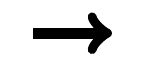
\begin{tikzpicture}
        \draw[->,line width=4pt] (0,0) to (1,0);
      \end{tikzpicture}
      \begin{tikzpicture}
      \def\BACKGROUNDTWO{lightblue}
      \fill[\BACKGROUNDTWO] (2,0) rectangle ++ (1,1);
      \fill[\BACKGROUNDTWO] (3,0) rectangle ++ (1,1);
        \draw[step=1.0,gray,thin] (0,0) grid (1,1);
        \node[matrix of math nodes,anchor=south west,inner sep=0pt,
        nodes={draw,minimum size=1cm,anchor=center},
        column sep=-\pgflinewidth,row sep=-\pgflinewidth,font=\huge\ttfamily]
        {
        0 & 0  & 1 & 0 & 0 & 0 & 0 & 0\\
        };
      \end{tikzpicture}
    \end{adjustbox}
  }\caption{The result of our bit-shifting\index{shifting}, \icode{AND}'ing\, and \icode{OR}ing.}
\end{figure}

\subsection{Flipping the Byte's Position}
The remaining steps for the other two bit-pairs in the byte are similar. In the case of our
example they will have no effect as the result will be always be zero for them. We've
effectively mirrored our bitpair\index{bitpair} already.

The next and last thing we have to do with our mirrored byte is adjust it's position in the 8 byte sequence\index{sequence}
in the character\index{character} definition. In the example below we are dealing with a byte on
the left which occurs as the 5th position in the byte sequence\index{sequence} and in order to be
inverted\index{inverted} needs to be moved to the 4th position.

So whereas we were dealing with a left-right mirroring in the byte itself we are now dealing with an up-down
mirroring in the position of the byte in its sequence\index{sequence}. The total effect of our inversion operation is
to flip the character\index{character} set from left to righ and top to bottom:

\begin{figure}[H]
{
  \setlength{\tabcolsep}{3.0pt}
  \setlength\cmidrulewidth{\heavyrulewidth} % Make cmidrule = 
    \begin{adjustbox}{width=10cm,center}
  \begin{subfigure}{0.3\textwidth}
  \input{planets/planet1Charset_\$40_bits_2}
  \end{subfigure}
  \begin{subfigure}{0.3\textwidth}
  \input{planets/planet1Charset_\$40_bits_inv_2}
  \end{subfigure}
  \end{adjustbox}
}\caption[]{Flipping the piece both up to down, and left to right.}
\end{figure}

The second half of \icode{InvertCharacter\index{InvertCharacter}} that does this looks like:

\begin{lstlisting}[escapechar=\%]
      ; Now that the byte has been inverted%\index{inverted}%, invert the position in
      ; the 8 byte charset%\index{charset}% definition. For example, if the position is
      ; 0 then the inverted%\index{inverted}% position is 7.

      ; Mask out everything but the last 3 bits in the current upper
      ; planet%\index{planet}% position. 
      TYA
      PHA
      AND #$07
      TAY
      PLA
      PHA
      AND #$F8
      STA charSetDataPtrLo%\index{charSetDataPtrLo}%

      ; Now add the inverted%\index{inverted}% position to get the correct lower planet%\index{planet}%
      ; position in the 8-byte charset%\index{charset}% definition. charSetDataPtrLo%\index{charSetDataPtrLo}% is
      ; just temporary storage here. We store the final value for use
      ; by the calling routine%\index{routine}% in 'X' below.
      LDA positionInInvertedCharSet%\index{positionInInvertedCharSet}%,Y
      CLC
      ADC charSetDataPtrLo%\index{charSetDataPtrLo}%

      ; By storing the updated position in the charset%\index{charset}% definition
      ; to 'X' here, we're changing the offset used in 
      ; lowerPlanetSurfaceCharset%\index{lowerPlanetSurfaceCharset}% in InvertSurfaceDataForLowerPlanet%\index{InvertSurfaceDataForLowerPlanet}%.
      TAX

      PLA
      TAY
\end{lstlisting}

The key to this operation lies in the use of the array \icode{positionInInvertedCharSet\index{positionInInvertedCharSet}}.
If we know that the current byte is number 5 in the 8 byte sequence\index{sequence} (i.e. the red row
below):

\begin{figure}[H]
{
  \setlength{\tabcolsep}{3.0pt}
  \setlength\cmidrulewidth{\heavyrulewidth} % Make cmidrule = 
    \begin{adjustbox}{width=6cm,center}
  \begin{subfigure}{0.3\textwidth}
  \input{planets/planet1Charset_\$40_bits_2}
  \end{subfigure}
  \end{adjustbox}
}\caption[]{Byte 5 highlighted in red.}
\end{figure}

then we can use that as an index into \icode{positionInInvertedCharSet\index{positionInInvertedCharSet}}
to retreve the corresponding position in the inverted\index{inverted} character\index{character} set definition. As we can
see value of the the 5th byte in \icode{positionInInvertedCharSet\index{positionInInvertedCharSet}} is \icode{\$03}:

\begin{lstlisting}[escapechar=\%]
positionInInvertedCharSet%\index{positionInInvertedCharSet}%      .BYTE $07,$06,$05,$04,$03,$02,$01,$00
\end{lstlisting}

Which as we can see is the appropriate position for the byte in the inverted\index{inverted} character\index{character} set (the
4th byte or red row starting from the top). (Remember that our index into arrays starts at zero,
so an index value of zero will pick the first byte and of three, as in this case, will pick the fourth.)

\begin{figure}[H]
{
  \setlength{\tabcolsep}{3.0pt}
  \setlength\cmidrulewidth{\heavyrulewidth} % Make cmidrule = 
    \begin{adjustbox}{width=6cm,center}
  \begin{subfigure}{0.3\textwidth}
  \input{planets/planet1Charset_\$40_bits_inv_2}
  \end{subfigure}
  \end{adjustbox}
}\caption[]{Byte 5 when flipped.}
\end{figure}

So where do we get the position of the current byte in the uninverted character\index{character} set? This was
passed into \icode{InvertSurfaceDataForLowerPlanet\index{InvertSurfaceDataForLowerPlanet}} and \icode{InvertCharacter\index{InvertCharacter}} in the \icode{Y}
register\index{register}. It's a value between 0 and 256 which references the offset of the current byte
in the character\index{character} set data as a whole so all we have to do is clamp it to a value between 0 and 7
to get the value we need within the 8-byte definition for this specific character\index{character}.

\begin{lstlisting}[escapechar=\%]
      ; Mask out everything but the last 3 bits in the current upper
      ; planet%\index{planet}% position. 
      TYA
      PHA
      AND #$07
\end{lstlisting}

The clamping is achieved by the \icode{AND} statement. If we imagine that \icode{Y} has a value of
\icode{\$D4}, we transfer it to the \icode{A} register\index{register} (\icode{TYA} and then do an \icode{AND} operation
with \icode{\$07}:

\begin{figure}[H]
  {
    \setlength{\tabcolsep}{3.0pt}
    \setlength\cmidrulewidth{\heavyrulewidth} % Make cmidrule = 
    \begin{adjustbox}{width=10cm,center}

      \begin{tabular}{rllllllll}
        \toprule
        Byte & Bit 7 & Bit 6 & Bit 5 & Bit 4 & Bit 3 & Bit 2 & Bit 1 & Bit 0        \\
        \midrule
        \$D4 & 1 & 1 & 0 & 1 & 1 & 0 & 0 & 0 \\
        \$07 & 0 & 0 & 0 & 0 & 1 & 1 & 1 & 1 \\
        \midrule
        Result: \$04 & 0 & 0 & 0 & 0 & 1 & 0 & 0 & 0 \\
        \addlinespace
        \bottomrule
      \end{tabular}

    \end{adjustbox}

  }\caption*{AND'ing \$D4 and \$07 gives \$04.}
\end{figure}

This gives us \icode{\$04} as a result, which as we saw returns \icode{\$03} when used as an index
into \icode{positionInInvertedCharSet\index{positionInInvertedCharSet}}.

With our new position for the byte in the character\index{character} set definition established we can store it to the
\icode{X} register\index{register} and use that as the position in \icode{lowerPlanetSurfaceCharset\index{lowerPlanetSurfaceCharset}} where we will
store the \icode{invertedCharToDraw\index{invertedCharToDraw}} we calculated earlier. We do this when we return from the
\icode{InvertCharacter\index{InvertCharacter}} routine\index{routine} and are back in \icode{InvertSurfaceDataFor\-LowerPlanet\index{InvertSurfaceDataForLowerPlanet}}:

\begin{lstlisting}[escapechar=\%]
        JSR InvertCharacter%\index{InvertCharacter}%
        LDA invertedCharToDraw%\index{invertedCharToDraw}%
        ; Note that 'X' was updated by InvertCharacter%\index{InvertCharacter}%
        STA lowerPlanetSurfaceCharset%\index{lowerPlanetSurfaceCharset}%,X
\end{lstlisting}

With that done, we've added another brick in the wall. Or more precisely, another byte in the 
256 that in total make up the tileset for the upper and lower planets respectively. As the 
materialization sequence\index{sequence} proceeds we slowly fill out the tileset byte-by-byte. After a few
seconds we've successfully cheated our way into generating the lower planet\index{planet}'s tileset on the
fly into \icode{lowerPlanetSurfaceCharset\index{lowerPlanetSurfaceCharset}} and the game is ready to play.

\begin{figure}[H]
    \centering
      \includegraphics[width=6cm]{planets/entry_images/entry73.png}%
      \includegraphics[width=6cm]{planets/entry_images/entry255.png}%
\caption{The planets when we start the materialization sequence\index{sequence}, and when we end.}
\end{figure}
